\documentclass[12pt,nofoldmark,notumble]{leaflet}

\usepackage[T2A]{fontenc}
\usepackage[utf8]{inputenc}
\usepackage[russian]{babel}
\usepackage{graphicx}
\usepackage{xcolor}
\usepackage[most]{tcolorbox}
\usepackage{enumitem}
\usepackage{array}
\usepackage{float}
\usepackage{subcaption}

\setlength{\parindent}{0pt}
\setlength{\parskip}{2pt}
\setlist[itemize]{leftmargin=*, itemsep=1pt, topsep=1pt, label=\textbullet}
\pagestyle{empty}

\definecolor{maincolor}{RGB}{0,90,160}
\definecolor{accentcolor}{RGB}{230,120,20}

% ВАЖНО: убираем breakable
\newtcolorbox{sectionbox}[1]{
	colback=white,
	colframe=maincolor,
	fonttitle=\bfseries\large,
	title=#1,
	boxrule=0.7pt, arc=2pt,
	left=3pt, right=3pt, top=1pt, bottom=1pt,
	fontupper=\large,
	before skip=2pt, after skip=2pt
}
\newtcolorbox{notebox}[1]{
	colback=accentcolor!10,
	colframe=accentcolor,
	fonttitle=\bfseries\large,
	title=#1,
	boxrule=0.6pt, arc=2pt,
	left=3pt, right=3pt, top=1pt, bottom=1pt,
	fontupper=\large,
	before skip=2pt, after skip=2pt
}

\begin{document}

% ========== ПАНЕЛЬ 1 ==========
\begin{center}
	{\large\bfseries\color{maincolor} Neoclock}\\[2pt]
\end{center}
\hrule

\vspace{1cm}

\begin{sectionbox}{Краткое описание проекта}
	Настольные часы на ваккумно-люминимцентных индикаторах, способные
	отображать текущее время и дату. Часы оснащены двумя дисплеями,
	и кнопками для настройки.
\end{sectionbox}

\vspace{1cm}
\begin{notebox}{Авторы: состав команды и распределение задач}
	\begin{itemize}
		\normalsize
		\item Белокопытов Александр (Б01-507) --- проектирование
			корпуса,
			проектирование печатных плат, изготовление
			и сборка устройства.
		\item Мартынов Александр (Б01-505) --- схемотехника (проектирование
			схемы), проектирование печатных плат,
			изготовление и сборка устройства.
	\end{itemize}
\end{notebox}

\begin{figure}[H]
	\centering

	\begin{subfigure}{0.5\linewidth}
		\centering
		
\includegraphics[width=0.7\linewidth]{images/tg_channel_qr.pdf}
		\caption*{Telegram}
	\end{subfigure}%
	\begin{subfigure}{0.5\linewidth}
		\centering
		
\includegraphics[width=0.7\linewidth]{images/github_repo_qr.pdf}
		\caption*{GitHub}
	\end{subfigure}
\end{figure}

% ========== ПАНЕЛЬ 2 ==========
\newpage
\begin{sectionbox}{Основные электронные компоненты}
	\textbf{Сенсоры:}\\
	Три кнопки, фоторезистор, датчик температуры и влажности.
	\vspace{0.3cm}

	\textbf{Контроллер:}
	\begin{enumerate}
		\item Микроконтроллер: ESP32
		\item Драйвер: ULN2003, 74HC595
		\item Преобразователь: pwm boost power supply
	\end{enumerate}

	\textbf{Актуаторы:}\\
	Отображение текущего времени и даты, испускание звукового сигнала
	по заданному времени, режим секундомера, автономный ход часов
	в отсутствие электропитания.
\end{sectionbox}

\vspace{1cm}

\begin{sectionbox}{Дополнительные технические характеристики}
	\begin{itemize}
		\item Питание: 5V DC
		\item Потребление: $\sim$ 500 mA
		\item Габариты: 100$\times$100$\times$90
		\item Интерфейсы связи: кнопки, шнур питания (или USB
			разьем)
	\end{itemize}
\end{sectionbox}

% ========== ПАНЕЛЬ 3 ==========
\newpage
\begin{sectionbox}{Управление и индикация}
	\textbf{Управление:}\\
	Управление устройством осуществляется посредством кнопок,
	позволяющих осуществлять навигацию по меню и изменение настроек.
	\vspace{0.3cm}

	\textbf{Отображение информации:}\\
	Для отображения информации используются 2 вакуумно-люминисцентных
	индикатора, имеющих семисегментные разряды и мнемонические знаки.
\end{sectionbox}

\vspace{2cm}

\begin{sectionbox}{Основная инженерная задача}
	\normalsize
	\begin{itemize}
		\item Используя общедоступную и современную элементарную
			базу успешно запустить вакуумно-люминисцентные
			ретро-индикаторы
		\item Собрать устройство, используя преимущественно
			технологии \textit{физтех-фабрики}, собственные
			знания и умения из соответствующих областей
			(физика, радиотехника, системное
			программирование)
		\item Получить от изготовления проекта \textit{максимум}
			инженерных знаний и опыта
	\end{itemize}
\end{sectionbox}

\newpage

\begin{sectionbox}{Функциональная схема устройства}
	\begin{figure}[H]
		\centering
		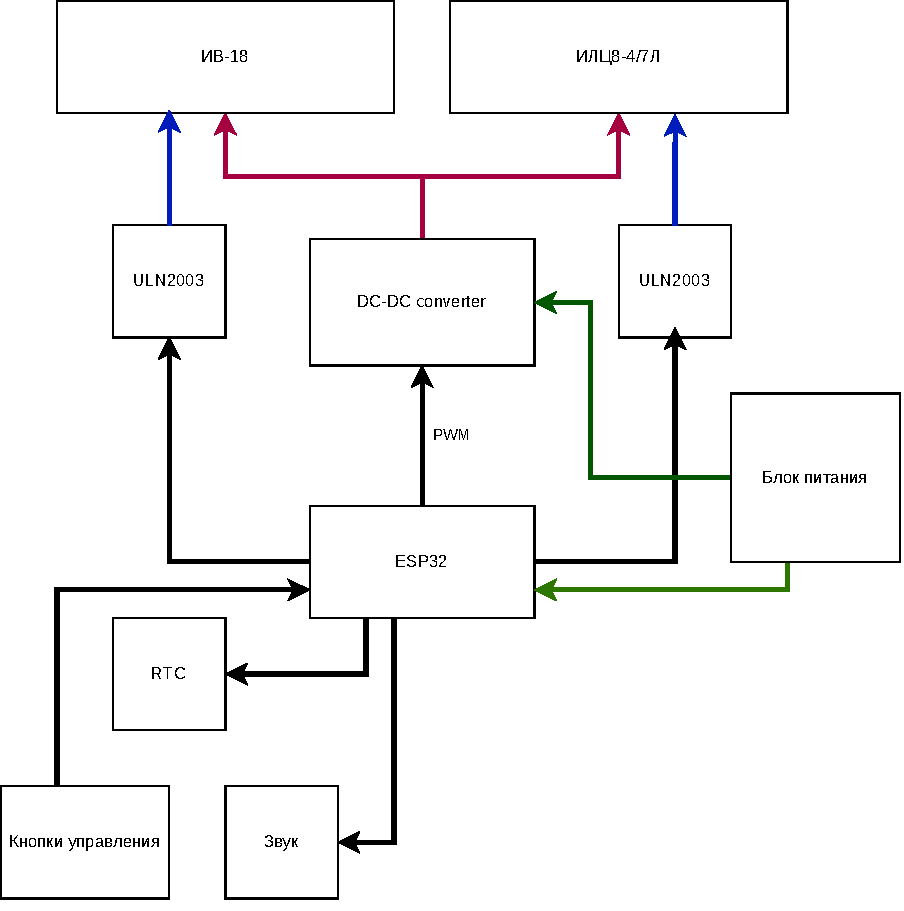
\includegraphics[width=\linewidth]{images/block_scheme.pdf}
	\end{figure}
\end{sectionbox}

\begin{sectionbox}{Прогресс проекта}
	\textbf{Было заявлено:}
	\begin{itemize}
		\item Собрать прототип преобразователя питания на
			макетной плате
		\item Спроектировать и изготовить плату для прототипа
		\item Запустить дисплеи
		\item Написать API для дисплея, собрать минимально
			рабочий прототип схемы, изготовить корпус на 3D
			принтере
	\end{itemize}

	\textbf{Выполнено:}
	\begin{itemize}
		\item Собран и отлажен прототип преобразователя питания
			на макетной плате
		\item Спроектирована и изготовлена плата для прототипа
		\item Запущены дисплеи
		\item Написан API для дисплея, собран минимально
			рабочий прототип схемы, изготовлен корпус часов
			из оргстекла
	\end{itemize}

	\textbf{Осталось:}
	\begin{itemize}
		%TODO
		\item Дописать программную часть
		\item Опциональная часть
	\end{itemize}
\end{sectionbox}

\begin{sectionbox}{Визуализация}
	\begin{figure}[H]
		\centering
		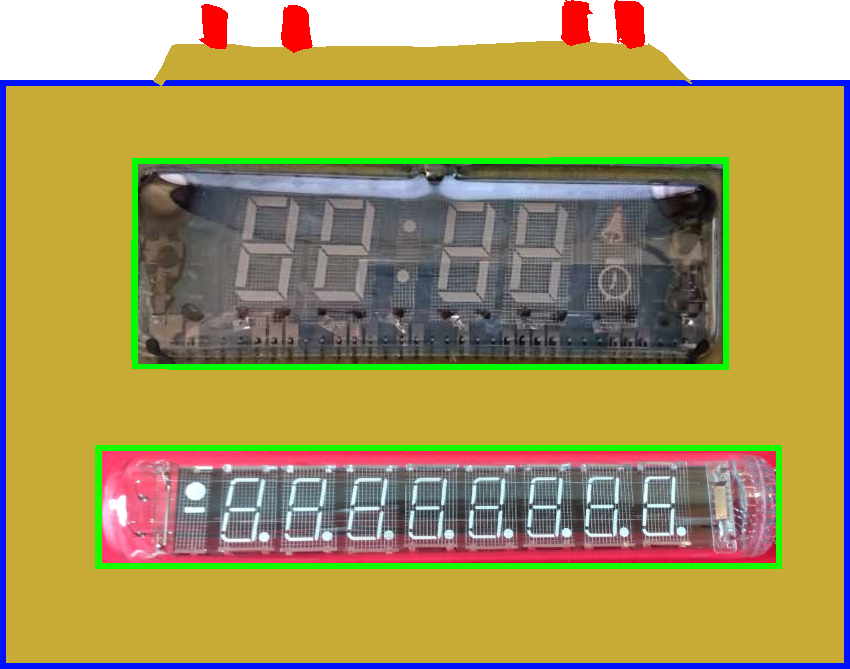
\includegraphics[width=\linewidth]{images/draft.pdf}
		\caption*{Эскиз}
	\end{figure}

	\vspace{2cm}

	\begin{figure}[H]
		\centering
		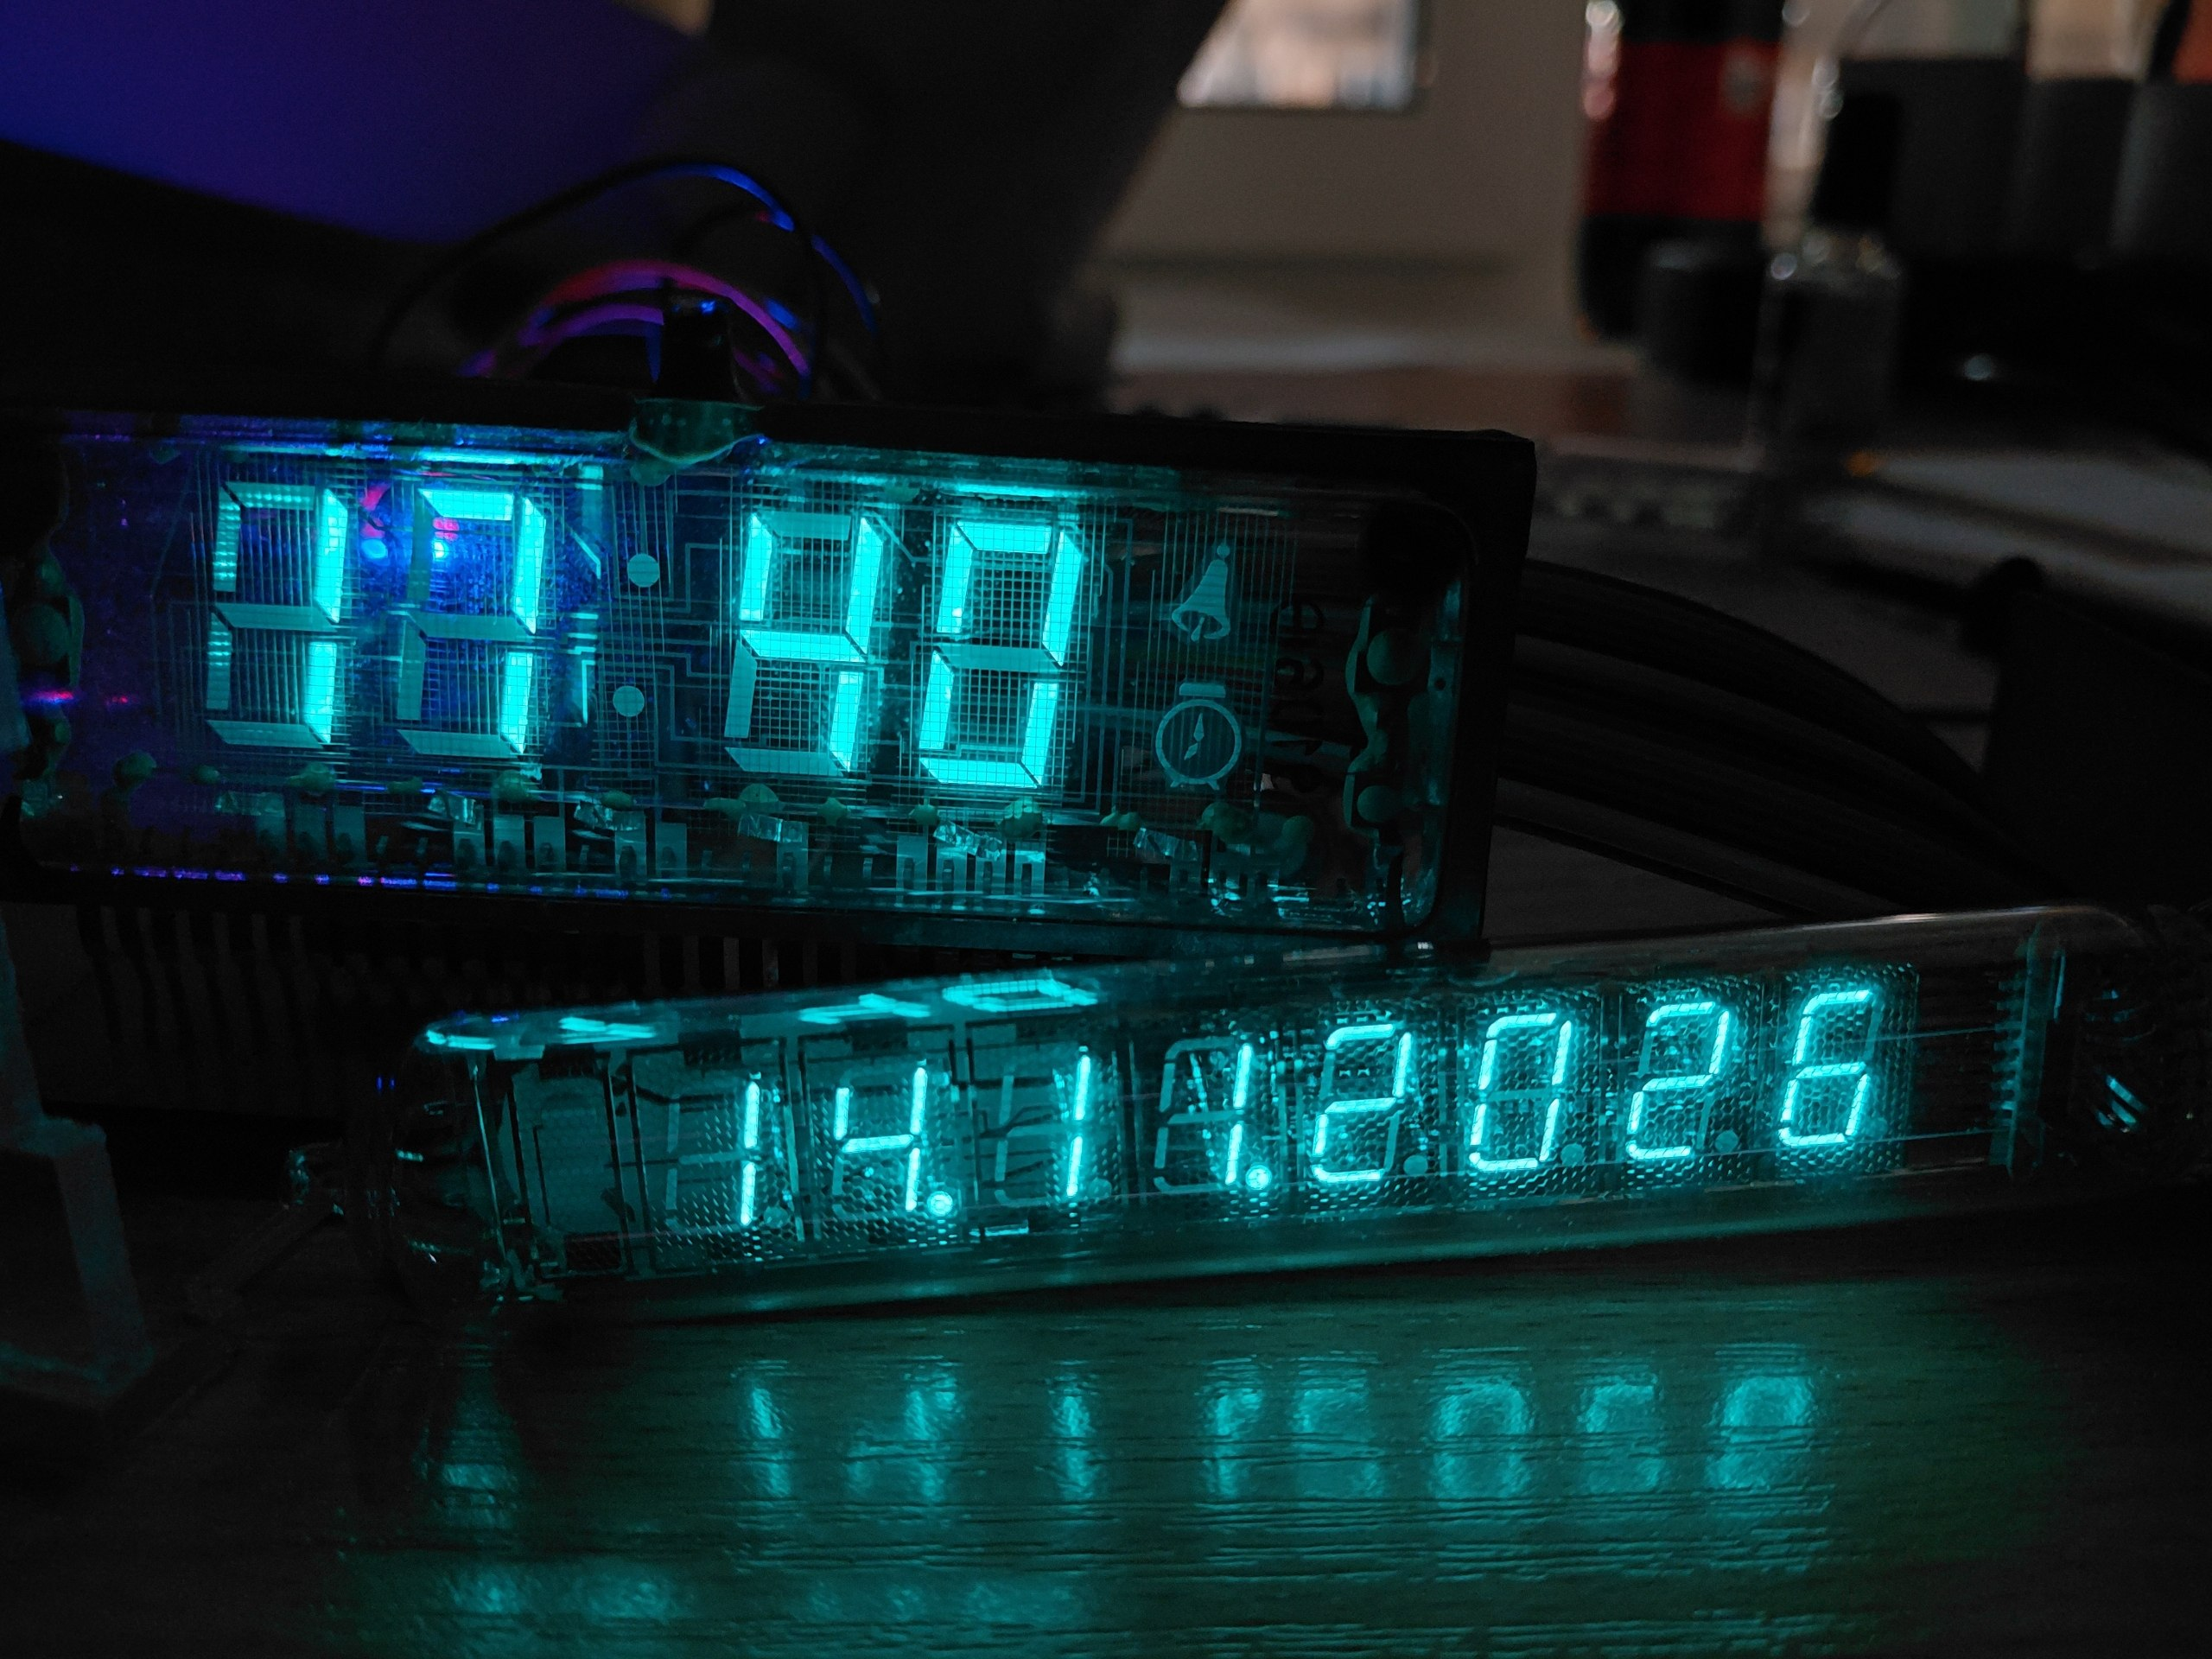
\includegraphics[width=\linewidth]{images/working_clocks.jpg}
		\caption*{Собранный прототип}
	\end{figure}
\end{sectionbox}

\end{document}
